\chapter{Оценка корреляционных функций}

Рассмотрим задачу оценки корреляционных функций (КФ) на примере оценки автокорреляционной функции (АКФ). АКФ, по определению, представляет неслучайную функцию.
Для получения данной функции необходимо обладать бесконечным количеством реализаций или, в случае эргодического процесса, реализацией бесконечной длинны \cite{bolshakov-book}.

Оценка АКФ ${\hat{r}_{xx}(\tau, T)}$ является случайной функцией. Оценка данной функции должна наилучшим образом отражать реальные характеристики процесса.

Из большого числа методов оценки АКФ наиболее часто применяются прямые и косвенные. При использовании прямого метода вычисляется интеграл:
\begin{equation}
	\label{eq:acf_integral_basic}
	\hat{r}_{xx}(\tau, T) = \frac{1}{T-\tau} \int_{0}^{t-\tau} (x(t) - \hat{E}(x))(x(t+\tau) - \hat{E}(x))dt,
\end{equation}
где ${\hat{r}_{xx}(\tau, T)}$ -  оценка автокорреляционной функции. Остальные методы: основанные на интегральном преобразовании Фурье, использующие интеграл вероятностей, принцип
знакосочетаний, компенсации, интерференции, разложения по ортогональным функциям, относятся к косвенным \cite{bolshakov-book}.

Погрешности можно разделить на три группы \cite{bolshakov-book}:
\begin{enumerate}
	\item Методические погрешности. Данные погрешности обусловлены ограниченностью отрезка реализации, шагом дискретизации и шумом квантования;
	\item Инструментальные погрешности. Данный вид погрешностей обусловлен погрешностями: измерительных приборов, записи, храниения, вычислений;
	\item Погрешности от влияния коррелированных и некоррелированных помех.
\end{enumerate}

В данной главе предлагается подхот к компенсации всех приведенных погрешностей. В конце главы представлено численное моделирование.

%%%%%%%%%%%%%%%%%%%%%%%%%%%%%%%%%
\section{Повышение точности оценки автокорреляционной функции}
Для эффективного использования АР-метода необходимо иметь точную оценку АКФ. Наличие шума в аддитивной смеси ведет к неточной
оценке АКФ, что, в свою очередь, ведет к смещенной оценке резонансных частот.

Подходы к компенсации шума при АР анализе достаточно подробно рассмотрены в классических работах \cite{kay_ar_book, kay_noise_compensation}.
При наличии АБГШ во входной смеси ${x(m)}$ ее АКФ может быть записана как:
\begin{equation}
	\label{eq:acf_noise_basic}
	r_{xx}(m) =	\begin{cases}
				r_{ss}(0) + \sigma_n^2, & \mbox{если } k=0 \\
				r_{ss}(m), & \mbox{если } k \ne 0.
			\end{cases}
\end{equation}

Если вычесть ${\sigma_n^2}$ из ${r_{xx}(0)}$ параметры АР процесса могут быть найдены. Однако, если ${\sigma_n^2}$ достаточно велика или 
оценка ${{\bf{\hat{R}_{xx}}}}$ плохая, матрица ${{\bf{\hat{R}_{xx}}} - {\bf{I}}\sigma_n^2}$ может быть не положительно определена. В данном
случае необходимо вводить поправочный коэффициент. Но для применения данного метода необходимы априорные знания или оценка ${\sigma_N^2}$,
что в случае оценки параметров ШПС в городских условиях является крайне затруднительным.

Различные методы оценки параметров для АР-модели, основанные на принципе максимального правдоподобия больше не
могут считаться ММП при наличии шума в данных. В виду сложности использования ММП, предложено несколько 
субоптимальных оценок \cite{marpl_book, kay_ar_book}:
\begin{enumerate}
	\item Применение АРСС;
	\item Фильтрация данных для уменьшения мощности шума;
	\item Компенсация параметров АР или оценки коэффициентов отражения;
	\item Использования АР-модели более высокого порядка.
\end{enumerate}

Разрешающая способность оценки частоты при применении АР-модели снижается при снижении уровня ОСШ. Разрешающую способность оценки АР-модели для гармонических сигналов
одинаковой мощности в случае известной АКФ можно определить приблизительно с помощью формулы Марпла \cite{marpl_book, kay_ar_book}:
\begin{equation}
	\label{eq:lpc_est_quality_1}
	F = \frac{1.03}{Tp[R_e(P+1)]^{0.31}},
\end{equation}
где ${F}$ - разрешение в герцах, ${T}$ - интервал отсчетов в секундах, ${P}$ - порядок модели, ${R_e}$ - ОСШ для отдельного гармонического сигнала, выраженный в линейных единицах.

В \cite{lacoss_spectral_est, chen_spectral_est, marple_1977} приведены исследования подтверждающие данное поведение.

В приведенных работах не рассмотрен еще один интересный алгоритм уточнения АКФ - итеративный пересчет АКФ. В данной работе используется
модификация данного алгоритма поэтому целесообразно рассмотреть его подробнее.

%%%%%%%%%%%
\section{Алгоритм итеративного вычисления АКФ}
\label{sec_ostanin}
В \cite{ostanin_akf} предлагается использовать метод последовательного вычисления АКФ для уточнения оценки АКФ. Данный метод
заключается в последовательном вычислении АКФ от АКФ несколько раз. При этом ОСШ увеличивается от итерации к итерации.
Процесс повторяется несколько раз. Количество итераций зависит от значения ОСШ сигнала. Возможность применения данного подхода в оценке параметров ШПС рассмотрена
автором в \cite{my_acf_cdma}.

Пусть входная смесь может быть записана как сумма полезного сигнала ${s(t)}$ и шума ${n(t)}$:
\begin{equation}
	\label{eq:acf_signal}
	x(t) = A \cos{(\omega t)} + n(t)
\end{equation}

Пусть функции ${s(t)}$ и ${n(t)}$ - центрированы. Тогда АКФ выражения \ref{eq:acf_signal} может быть записана как \cite{book_max}:
\begin{eqnarray}
	\label{eq:acf_rss_signal}
	r_{xx}(\tau)	& = & \lim_{T \to \infty} \frac{1}{T} \int \limits_0^T x(t)x(t-\tau)dt = \nonumber \\
			& = & \lim_{T \to \infty} \frac{1}{T} \int \limits_0^T (A \cos{(\omega t)} + n(t))(A \cos{(\omega t - \tau)} + n(t - \tau))dt
\end{eqnarray}

Тогда, оценка АКФ может быть записана как:
\begin{equation}
	\label{eq:acf_rss_signal_full}
	\hat{r}_{xx}(\tau)=\hat{r}_{ss}(\tau)+\hat{r}_{sn}(\tau)+\hat{r}_{ns}(\tau) + \hat{r}_{nn}(\tau)
\end{equation}

Корреляционные функции ${\hat{r}_{xn}}$ и ${\hat{r}_{nx}}$ тождественно равны 0, с точностью до погрешности, при условии независимости
${x(t)}$ и ${n(t)}$. Таким образом \ref{eq:acf_signal} можно переписать:
\begin{equation}
	\label{eq:acf_rss_signal_new}
	\hat{r}_{xx}(t) = \hat{r}_{ss}(t) + \epsilon (t)
\end{equation}
Стоит учесть, что ${\epsilon (t)}$ стремится к нулю с ростом ${T}$. Фурье-образ ${\hat{r}_{xx}(t)}$
представляет собой СПМ, а следовательно равен квадрату Фурье-образа исходной функции ${x(t)}$.
Если обозначить ОСШ, выраженное в линейных единицах, сигнала ${x(t)}$ как ${R_s}$, тогда ОСШ после вычисления АКФ может быть вычислено
как \cite{book_max}:
\begin{equation}
	\label{eq:acf_snr_est}
	R_e=2BTR_s \frac{1}{2+1/R_s}
\end{equation}

Стоит отметить, что функция ${\epsilon(\tau)}$, как и ${n(t)}$ - является центрированной и
стационарной случайной величиной.
Учитывая что гармоническая составляющая содержится в ${\hat{r}_{ss}(t)}$, а аддитивный шум в ${\epsilon(\tau)}$, можно провести
следующую итерацию вычисления АКФ. Для оценки ОСШ по формуле \ref{eq:acf_snr_est} нужно принять ${R_s' = R_e}$.

Из \ref{eq:acf_snr_est} видно, что увеличение ОСШ при вычислении оценки АКФ пропорционально ${2BT}$ и зависит от
ОСШ на входе коррелометра, так же можно отметить, что увеличение ОСШ происходит только при условии ${BT > \frac{1}{2R_s} + 1}$.

Так же можно получить оценку АКФ на ${N}$ - шаге. На Рис. \ref{pic:acf_0_iter} представлен входной сигнал, а на
Рис. \ref{pic:acf_1_iter}, \ref{pic:acf_4_iter} представлены оценки АКФ на шагах с 1 и 4.
Моделирование проводилось для гармонического сигнала при ОСШ -44 дБ с нормированной частотой 20 Гц для
отрезка 600 точек.

\begin{figure}[h]
	\center\scalebox{1}{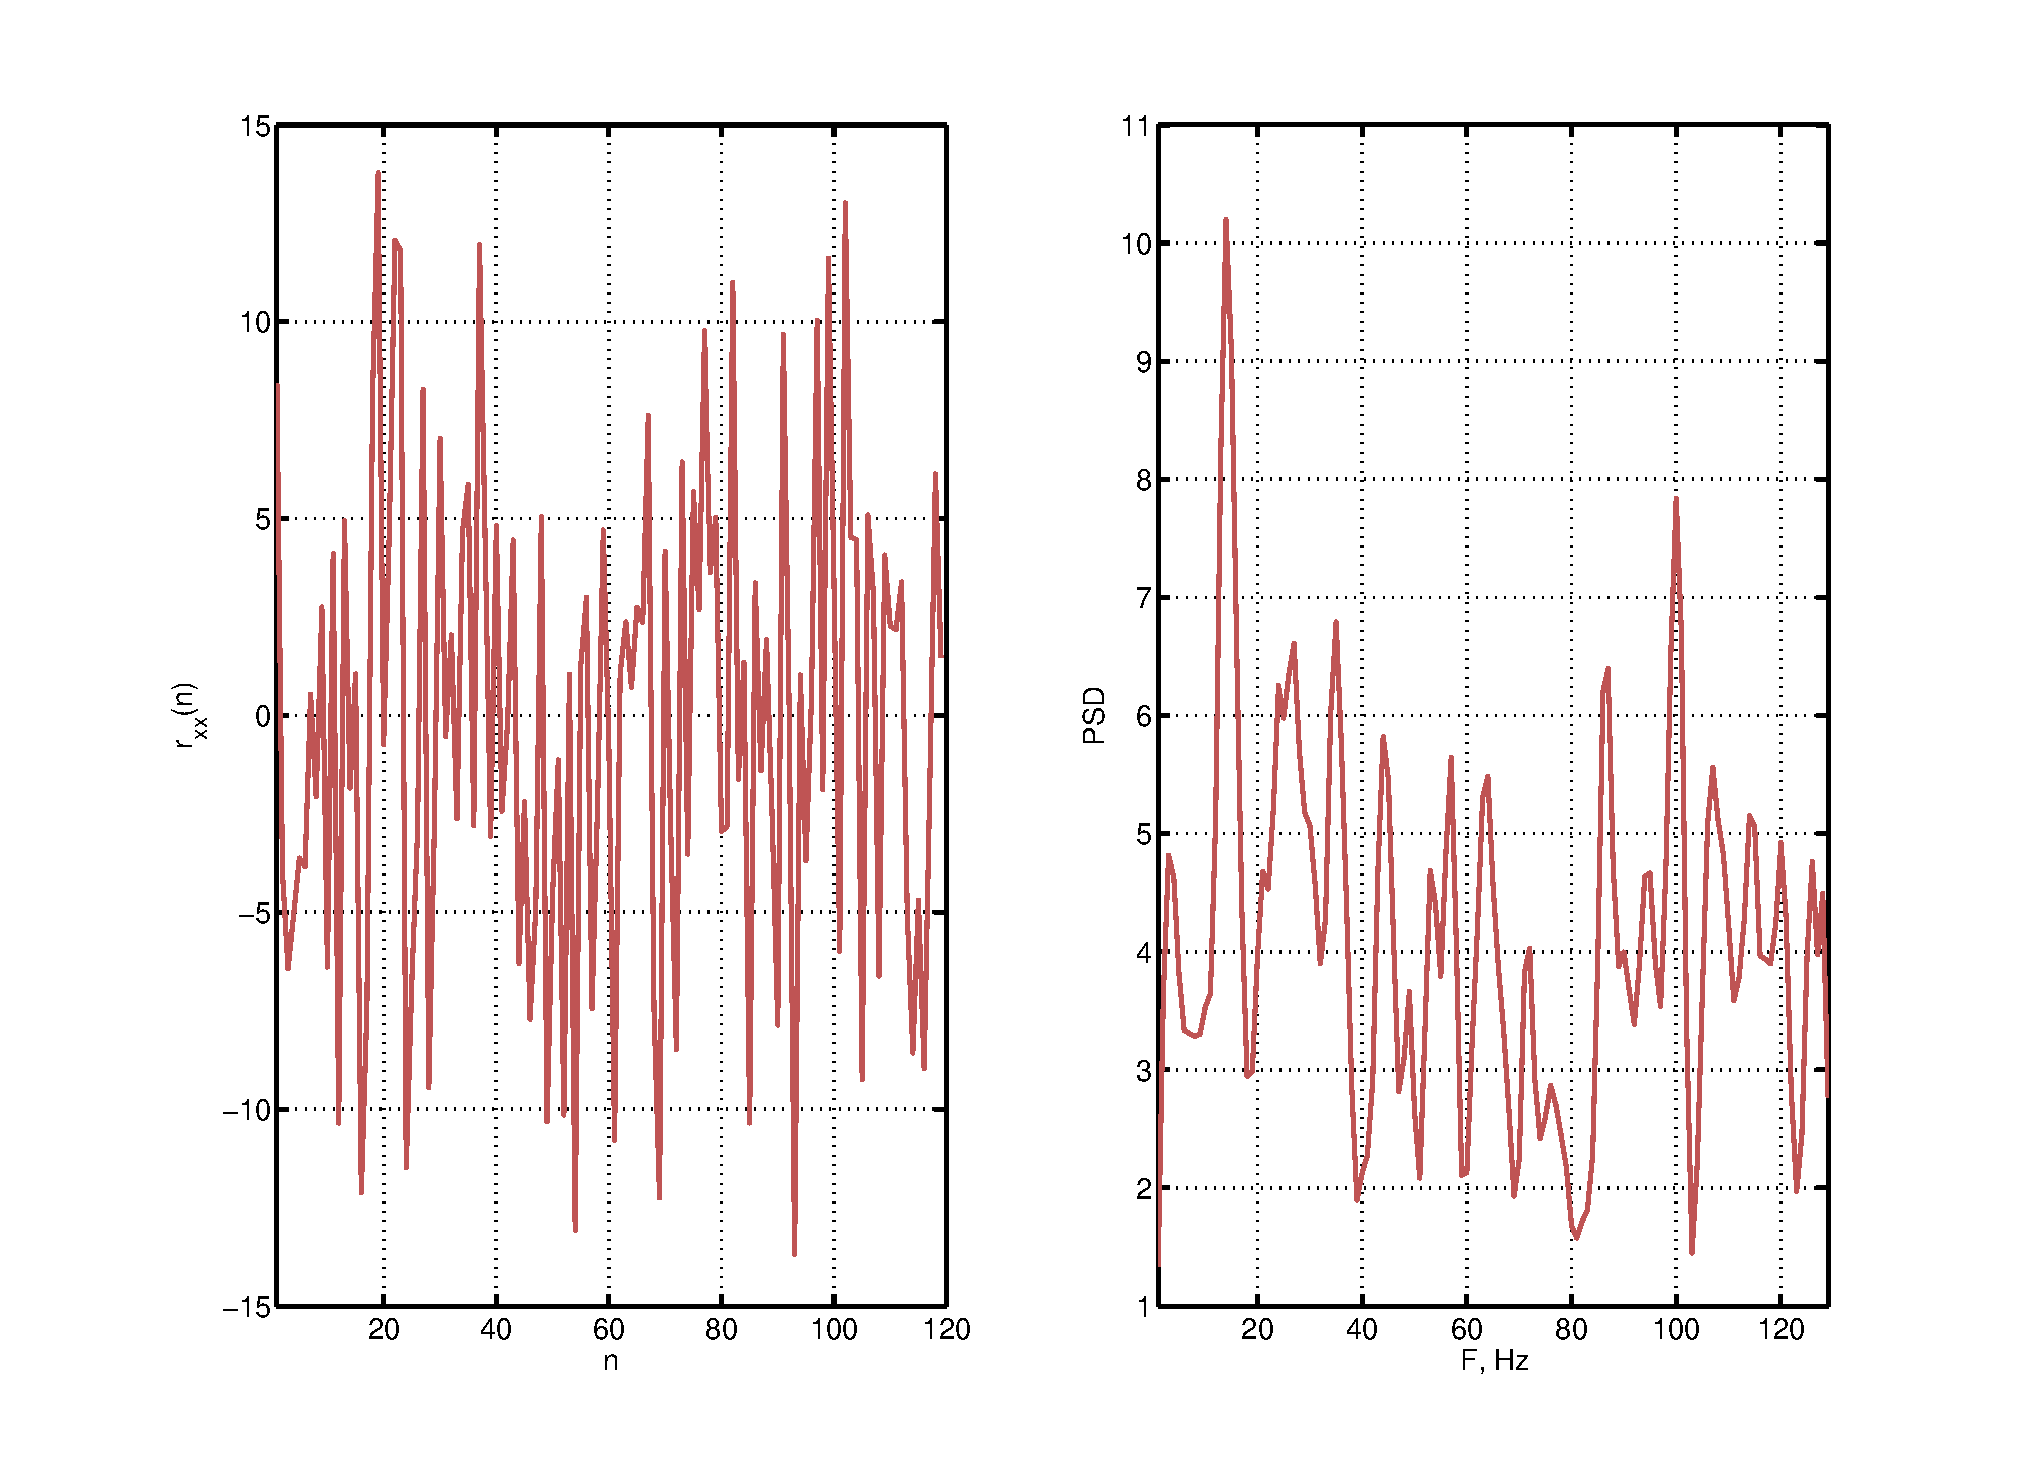
\includegraphics[width=1\linewidth]{acf_0_iter.eps}}
	\caption{Исходный сигнал и его спектр.}
	\label{pic:acf_0_iter}
\end{figure}

\begin{figure}[h]
	\center\scalebox{1}{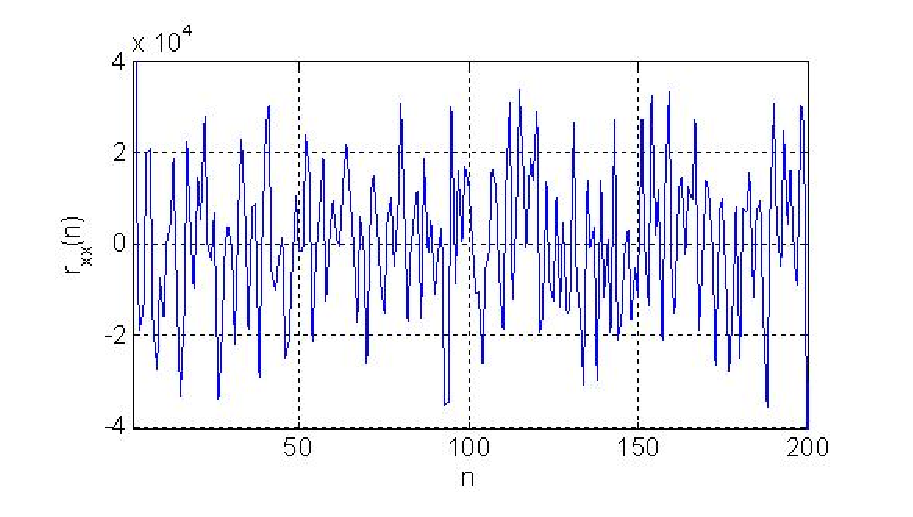
\includegraphics[width=1\linewidth]{acf_1_iter.eps}}
	\caption{Оценка АКФ на 1 итерации и ее спектр.}
	\label{pic:acf_1_iter}
\end{figure}

\begin{figure}[h]
	\center\scalebox{1}{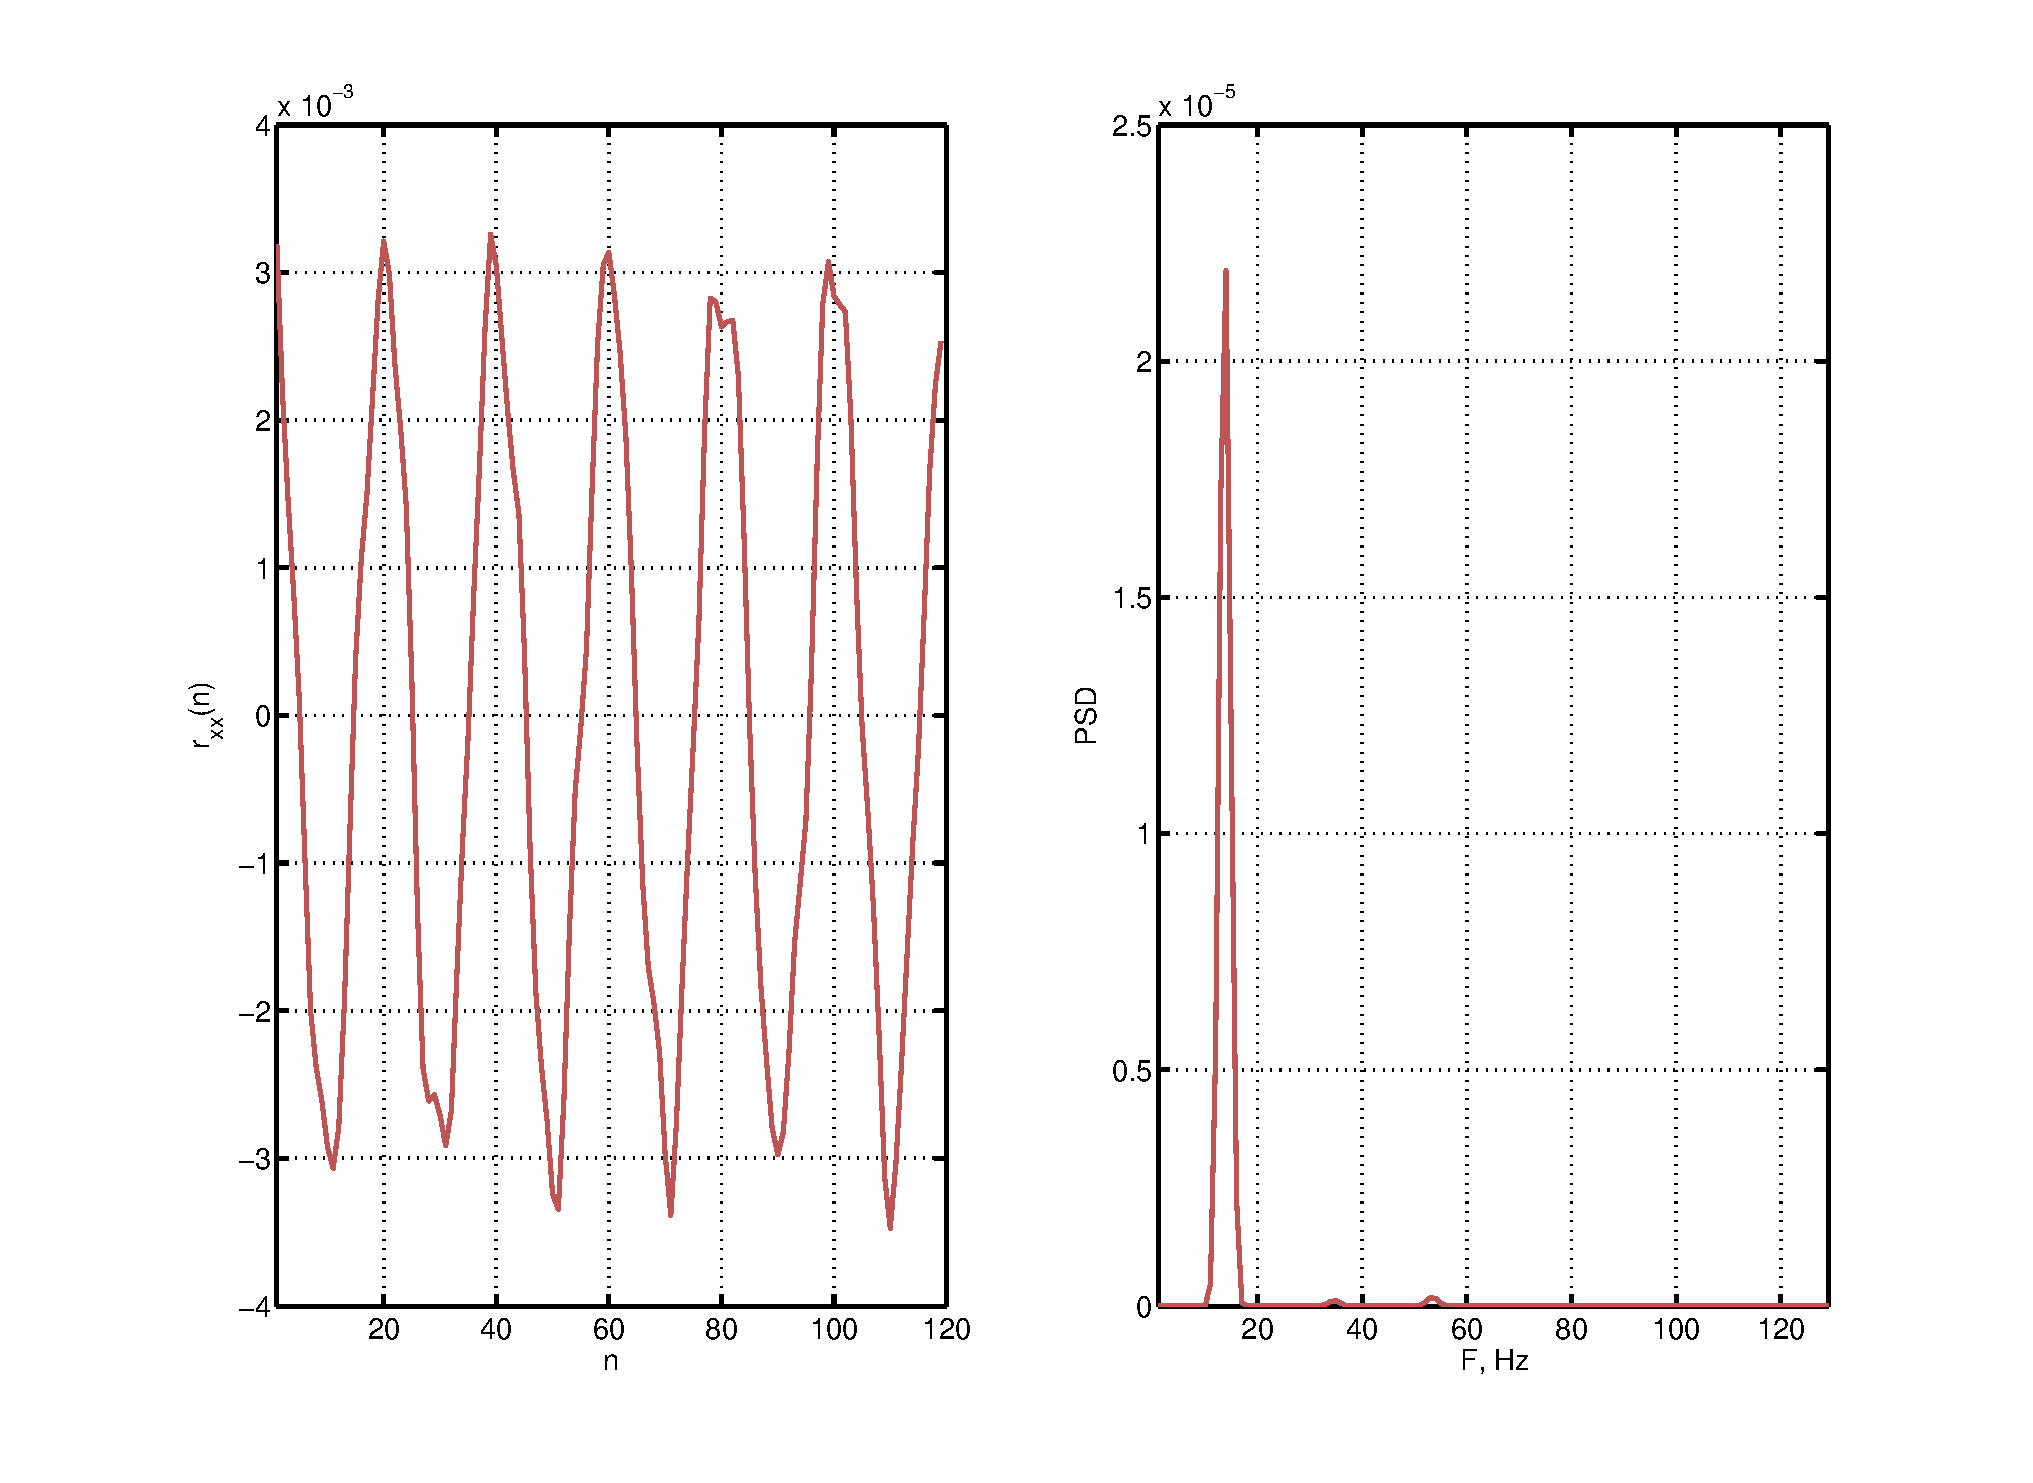
\includegraphics[width=1\linewidth]{acf_4_iter.eps}}
	\caption{Оценка АКФ на 4 итерации и ее спектр.}
	\label{pic:acf_4_iter}
\end{figure}

Представленный алгоритм позволяет значительно улучшить оценку АКФ. Следует отметить, что итеративный алгоритм вычисления АКФ так же
может быть использован для эффективного подавления окрашенного шума. В случае наличия интерференционной помехи в сигнале это дает
возможность получить несмещенную оценку частоты.

%%%%%%%%%%%%%%%%%
\section{Усовершенствованный итеративный алгоритм получения АКФ}
\label{sec_acf_fft}
Для приемников реального времени алгоритм, представленный в \cite{ostanin_akf} и приведенный в \ref{sec_ostanin}, применять при оценке 
частоты ШПС не представляется возможным в виду большого количества операций при вычислении АКФ.

Автором в \cite{my_acf} был предложен способ оптимизации алгоритма последовательного вычисления АКФ.
Для снижения вычислительных затрат указанный алгоритм предлагается реализовывать с использованием процедуры БПФ. 

Посчитаем АКФ для выражения \ref{eq:acf_signal}.
\begin{equation}
	\label{eq:lpc_akf_n}
	\hat{r}_{xx}(n) = \sum \limits_{k=1}^{K} x(k)x(k+n) = \frac{A^2}{2} \cos{(\omega{n})} + \Delta_n \delta{(n)} + \mu{(n)}
\end{equation}

Здесь ${\Delta_n}$ - дисперсия шума ${n(k)}$, ${\mu{(n)}}$ - ошибка оценки АКФ, ${\delta{(n)}}$ - дельта-функция. Дисперсия ошибки
оценки ${\Delta_{\mu}}$ будет в ${K}$ раз меньше чем дисперсия ${\Delta_n}$ шума в принимаемом сигнале, где ${K}$ - интервал
осреднения оценки АКФ.

Используя оценку АКФ вместо исходной выборки, вновь получим оценку АКФ:
${r_{xx2}(n) = \frac{A^4}{8} \cos{(\omega n)} + \bar{N} \delta{(N)}}$,
где мощность шума оценки ${\bar{N}}$ - будет значительно меньше.

Амплитуда сигнала на итерации ${k}$ будет равна ${\frac{A^{2^k}}{2^{2^k-1}}}$. Увеличение отношения ОСШ по мощности можно
вычислить по уже приведенной формуле \ref{eq:acf_snr_est}. 

Таким образом алгоритм можно представить в следующем виде.

Введем следующие обозначения: ${\bf{x}}$ – вектор входной смеси после снятия ПСП, ${\bf{F}}$ – матрица прямого преобразования Фурье,
${\bf{F}^{-1}}$- матрица обратного преобразования Фурье.  Оценку АКФ на первом шаге можно получить следующим образом:
\begin{equation}
	\label{eq:akf_1}
	\hat{\bf{r}}_1 = \bf{F}^{-1}\left[ \bf{Fx} \cdot (\bf{Fx})^* \right] = \bf{F}^{-1} \left[ \left| \bf{Fx} \right| ^2 \right]
\end{equation}

Здесь знак ${(\cdot)}$  означает поэлементное перемножение векторов, ${\left| \bf{Fx} \right| ^2}$ - поэлементное возведение модуля комплексного числа в квадрат, ${*}$ -
комплексное сопряжение.  Следуя алгоритму, изложенному в \cite{ostanin_akf} вычислим оценку АКФ от ${\hat{\bf{r}}_1}$:
\begin{eqnarray}
	\label{eq:akf_2}
	\hat{\bf{r}}_2 & = & \bf{F}^{-1}\left[ \bf{F} \hat{\bf{r}}_1 \cdot (\bf{F} \hat{\bf{r}}_1)^* \right] = \nonumber \\
		& = & \bf{F}^{-1}	\left[ 
				\bf{FF}^{-1} \left[
						\left| \bf{Fx} \right| ^2
					\right]
						\cdot \left( \bf{FF}^{-1} \left[ \left| \bf{Fx} \right| ^2 \right]
					\right) ^*
			\right] = \nonumber \\
		& = & \bf{F}^{-1} \left[ \left| \bf{Fx} \right| ^2 \cdot \left[ \left| \bf{Fx} \right| ^2 \right] ^* \right] =  \nonumber \\
		& = & \bf{F}^{-1} \left[ \left| \bf{Fx} \right| ^4 \right]
\end{eqnarray}

Рассуждая аналогично, можно показать, что уточненная оценка АКФ на ${K}$-ом шаге алгоритма, рассмотренного в \cite{ostanin_akf}
может быть получена без использования итераций с помощью выражения:
\begin{equation}
	\label{eq:akf_3}
	\hat{\bf{r}}_K = \bf{F}^{-1}\left[ \left| \bf{Fx} \right| ^{2^K} \right]
\end{equation}

Схематически алгоритм получения уточненной оценки АКФ на третьем шаге представлен на Рис. \ref{pic:akf_pic}.

\begin{figure}[h]
	\center\scalebox{0.8}{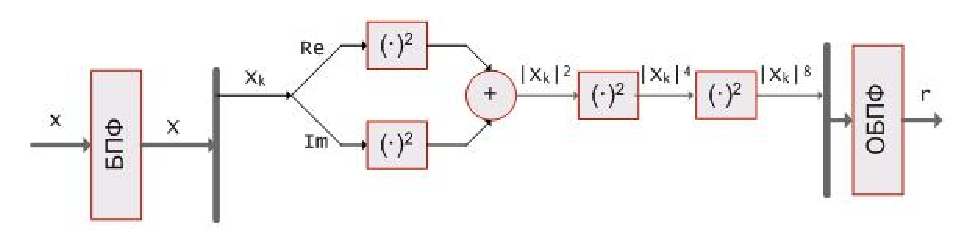
\includegraphics[width=1\linewidth]{akf_fft.eps}}
	\caption{Усовершенствованный итеративный алгоритм получения АКФ}
	\label{pic:akf_pic}
\end{figure}

Количество умножений действительных чисел необходимых для оценки АКФ прямым методом: 
\begin{equation}
	\label{eq:num_of_op_acf}
	OP_{ACF}=kN^2,
\end{equation}
где ${k}$  – количество итераций.

\begin{enumerate}
\item ${4NlogN}$ - действительных умножений - преобразование Фурье;
\item ${2N}$ - вычисление модуля комплексного числа;
\item ${N}$ - действительных умножений для каждой итерации (возведение в квадрат);
\item ${4NlogN}$ - действительных умножений – обратное преобразование Фурье. 
\end{enumerate}

Окончательно получаем:
\begin{equation}
	\label{eq:num_of_op_acf}
	OP_{ACF\_FFT}=8NlogN + (k+2)N,
\end{equation}

\section{Применение оконного взвешивания для оценки СПМ}

Так как в реальных условиях присутствует неопределенность по частоте, а длинна анализируемого объема данных конечна, пик на ПЧ в спектральной области не будет
представлять дельта функцию. Для улучшения свойств оценки СПМ представляется возможным использовать функции окон ${w(n)}$ - операция оконного взвешивания.
Свойства различных окон подробно рассмотрены например в \cite{shahtarin-spectrum-book, bolshakov-book}.

Наиболее популярными окнами являются: прямоугольное (равномерное), Бартлетта (треугольное), Ханна (косинус-квадрат), Хемминга (приподнятый косинус).

Оконная функция симметричного прямоугольного окна представляется выражением:
\begin{equation}
	\label{eq:rect_window}
	 w(n) = \begin{cases}
		1, |n| \le M; \\
		0, \mbox{в остальных случаях}.
		\end{cases}
\end{equation}
\begin{figure}[h]
	\center\scalebox{1}{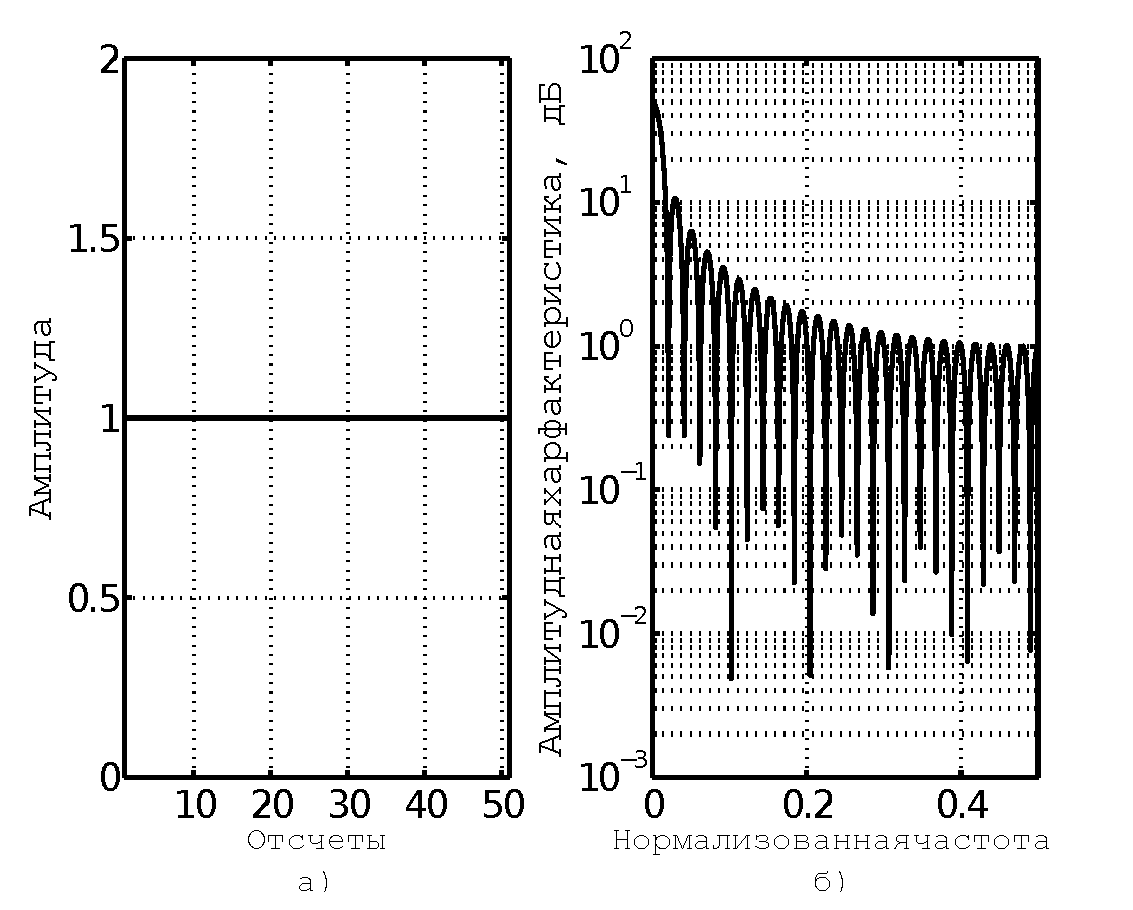
\includegraphics[width=1\linewidth]{various_windows_fig4.eps}}
	\caption{Прямоугольное окно. а - во временной области, б - в частотной}
	\label{pic:win_rect}
\end{figure}

Окно Бартлетта может быть представлено выражением:
\begin{equation}
	\label{eq:rect_bartlett}
	 w(n) = \begin{cases}
		1 - \frac{|n|}{M}, |n| \le M; \\
		0, \mbox{в остальных случаях}.
		\end{cases}
\end{equation}
\begin{figure}[h]
	\center\scalebox{1}{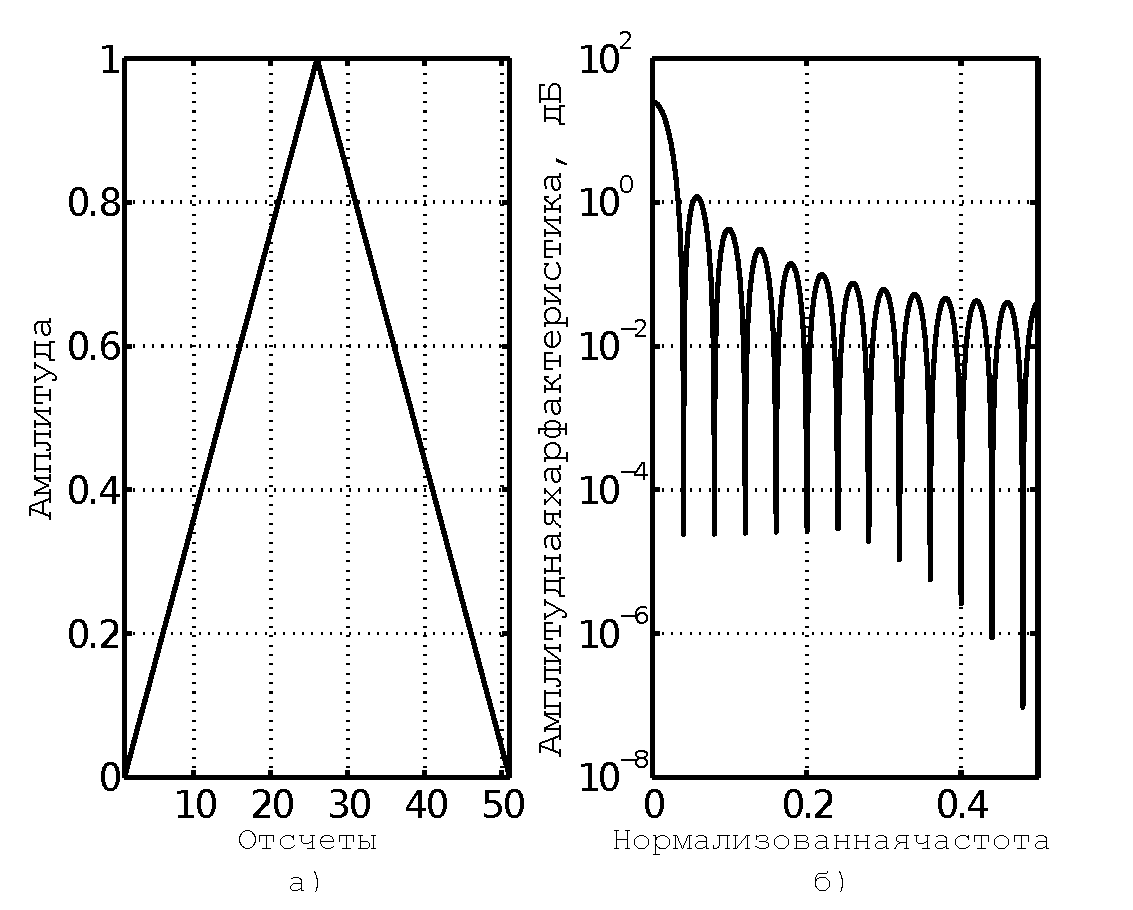
\includegraphics[width=1\linewidth]{various_windows_fig3.eps}}
	\caption{Окно Бартлетта. а - во временной области, б - в частотной}
	\label{pic:win_bart}
\end{figure}

Окно Хемминга может быть представлено выражением:
\begin{equation}
	\label{eq:rect_hamming}
	 w(n) = \begin{cases}
		0.54 - 0.46\cos \left( 2 \pi \frac{n}{M} \right), 0 \le n \le M; \\
		0, \mbox{в остальных случаях}.
		\end{cases}
\end{equation}
\begin{figure}[h]
	\center\scalebox{1}{\includegraphics[width=1\linewidth]{various_windows_fig2.eps}}
	\caption{Окно Хемминга. а - во временной области, б - в частотной}
	\label{pic:win_hamming}
\end{figure}

Окно Ханна может быть представлено выражением:
\begin{equation}
	\label{eq:rect_hann}
	 w(n) = \begin{cases}
		0.5 \left( 1 - \cos\left( 2 \pi \frac{n}{M} \right) \right) \\
		0, \mbox{в остальных случаях}.
		\end{cases}
\end{equation}

\begin{figure}[h]
	\center\scalebox{1}{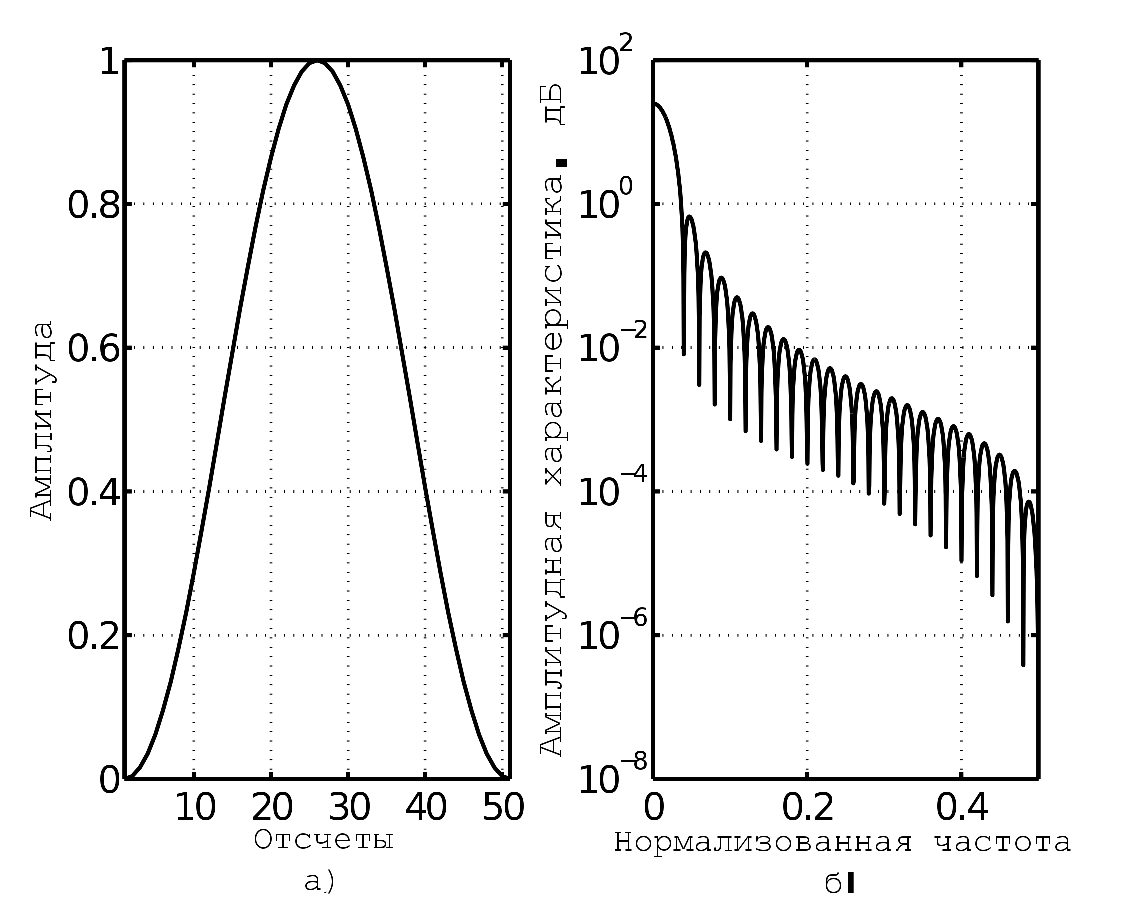
\includegraphics[width=1\linewidth]{various_windows_fig1.eps}}
	\caption{Окно Ханна. а - во временной области, б - в частотной}
	\label{pic:win_hann}
\end{figure}

Основными недостатками прямоугольного окна являются: наличие ложных максимумов, знакопеременность. В тоже время прямоугольное окно имеет самую малую ширину главного лепестка, но
одновременно с этим достаточно большие и медленно убывающие знакопеременные боковые лепестки. Окна Бартлетта и Ханна всюду положительны, а окно Хемминга положительно не всюду, однако
первый боковой лепесток составляет 0.021 высоты основного лепестка. Этим обусловлена популярность данного окна в задачах спектрального анализа.

В виду того, что рассмотренная в данной главе задача не является стандартной задачей спектрального анализа необходимо провести дополнительные исследования. В процессе
диссертационного исследования было проведено численное моделирование применения разных окон в процессе итеративного вычисления АКФ.

\section{Применение оконного взвешивания в задаче итеративного вычисления АКФ}

Из \cite{bolshakov-book} известно, что прямоугольное окно является самым узким, но вместе с тем имеет достаточно существенные боковые лепестки. В задаче итеративной оценки
АКФ, функция умножается несколько раз поточечно в частотном домене. Это позволяет предположить, что боковые лепестки будут увеличивать свое значение медленнее основного.
Для проверки данной гипотезы был проведен вычислительный эксперимент.

%%%%%%
\section{Практические аспекты применения}
\label{lab:sec2_windows}

При практической реализации алгоритма оценки частоты на основе АР-модели важным является качество оценки АКФ функции. В предложенном алгоритме итеаративной оценки АКФ,
в случае блочной обработки данных, будет наблюдаться эффект растекания спектра в следствии того, что ПЧ не является кратной частоте дискретизации. В процессе диссертационного
исследования было проведено численно моделирование применения различных комбинаций оконных функций и различных длин блоков нулей, при вычислении БПФ для повышения
разрешающей способности, как это рекомендовано для алгоритмов оценки СПМ \cite{bolshakov-book}.

Для оценки количества нулей, необходымых для получения оценки частоты в диапазон допустимой входной расстройки ФАПЧ был проведен вычислительный эксперимент. В качестве диапазона
ОСШ был взят диапазон от -30 дБ до 5 дБ, количество нулей в диапазоне ${[0, 6N]}$, где ${N}$ - длинна данных. Допустимая входная расстройка была взята в диапазоне ${[-40, 40]}$ Гц.
Опыт проводился на фоне АБГШ без МКИ. Оценивалось СКО оценки при использовании разных типов окон и разного количества итераций пересчета АКФ.

На Рис. \ref{pic:fft2_1} представлено моделирование для последовательности дополненной нулями до длинны ${2N}$ с применением различных оконных функций:
прямоугольного окна, окна Хемминга, окна Блекмана и окна Ханна при одной итерации уточнения АКФ.
\begin{figure}[h]
	\center\scalebox{0.8}{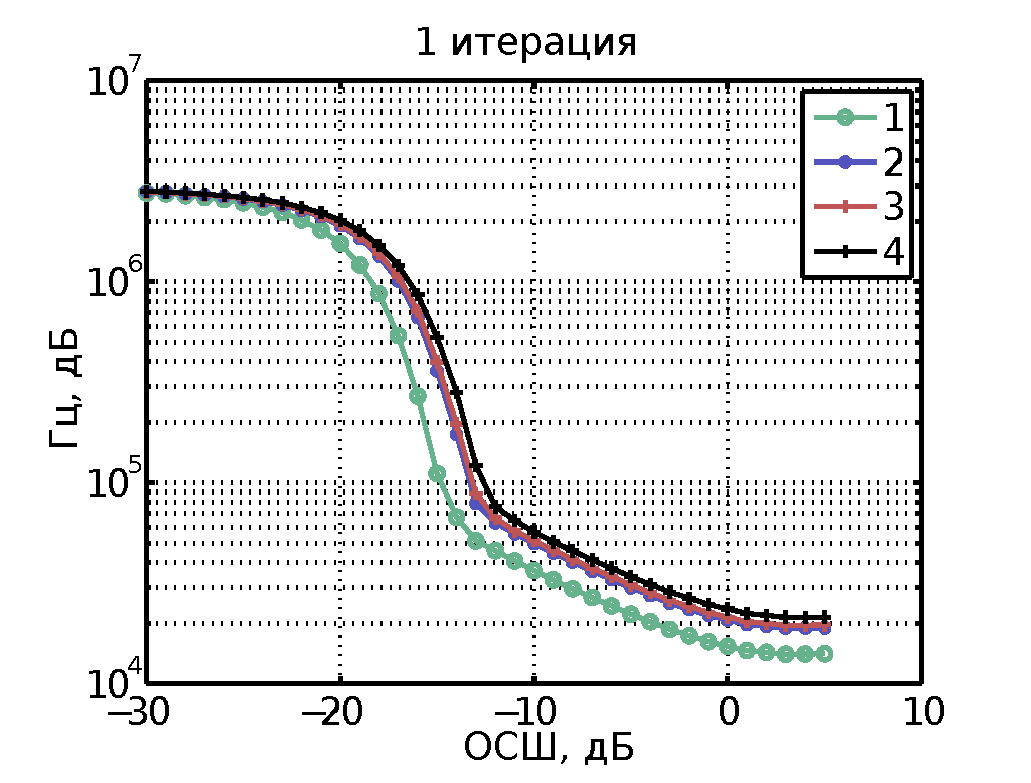
\includegraphics[width=1\linewidth]{fft2_1.eps}}
	\caption{СКО оценки частоты.\\1 - прямоугольное окно, 2 - окно Хемминга, 3 - окно Блекмана, 4 - окно Ханна.}
	\label{pic:fft2_1}
\end{figure}

На Рис. \ref{pic:fft2_2} представлено моделирование для последовательности дополненной нулями до длинны ${2N}$ с применением различных оконных функций:
прямоугольного окна, окна Хемминга, окна Блекмана и окна Ханна при двух итерациях уточнения АКФ.
\begin{figure}[h]
	\center\scalebox{0.8}{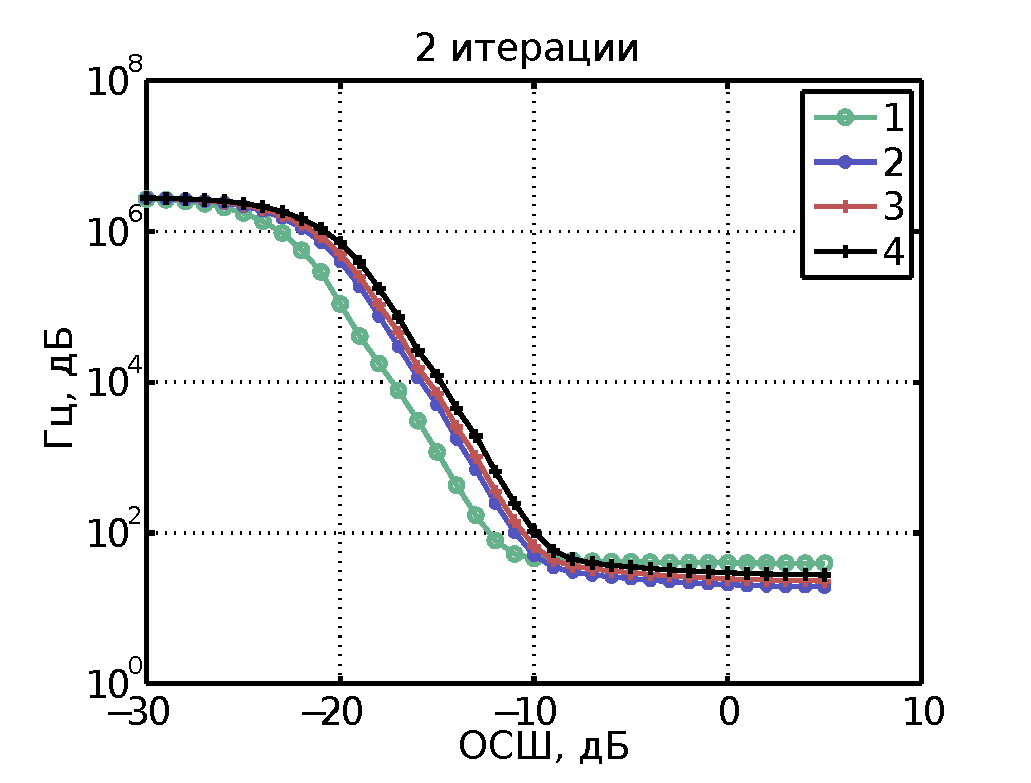
\includegraphics[width=1\linewidth]{fft2_2.eps}}
	\caption{СКО оценки частоты.\\1 - прямоугольное окно, 2 - окно Хемминга, 3 - окно Блекмана, 4 - окно Ханна.}
	\label{pic:fft2_2}
\end{figure}

На Рис. \ref{pic:fft2_3} представлено моделирование для последовательности дополненной нулями до длинны ${2N}$ с применением различных оконных функций:
прямоугольного окна, окна Хемминга, окна Блекмана и окна Ханна при трех итерациях уточнения АКФ.
\begin{figure}[h]
	\center\scalebox{0.8}{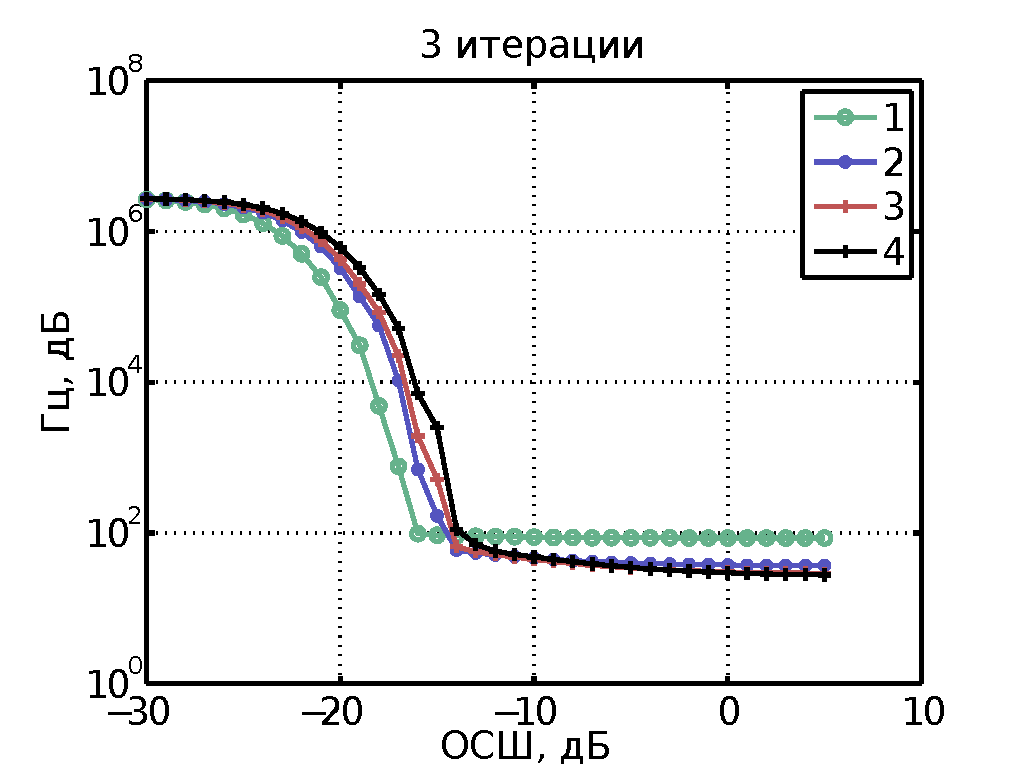
\includegraphics[width=1\linewidth]{fft2_3.eps}}
	\caption{СКО оценки частоты.\\1 - прямоугольное окно, 2 - окно Хемминга, 3 - окно Блекмана, 4 - окно Ханна.}
	\label{pic:fft2_3}
\end{figure}

Из Рис. \ref{pic:fft2_1}, \ref{pic:fft2_2}, \ref{pic:fft2_3} видно, что лучшие результаты показывает подход с применением прямоугольного окна. На Рис. \ref{pic:fft2_rect_1_2_3}
представлен график СКО оценки частоты для одной, двух и трех итераций уточнения АКФ с применением прямоугольного окна. Из графиков видно, что большее
количество итераций уточнения позволяет более точно получать оценку на низких ОСШ, вместе с тем точность оценки несколько снижается для ОСШ выше - 10 дБ.
\begin{figure}[h]
	\center\scalebox{0.8}{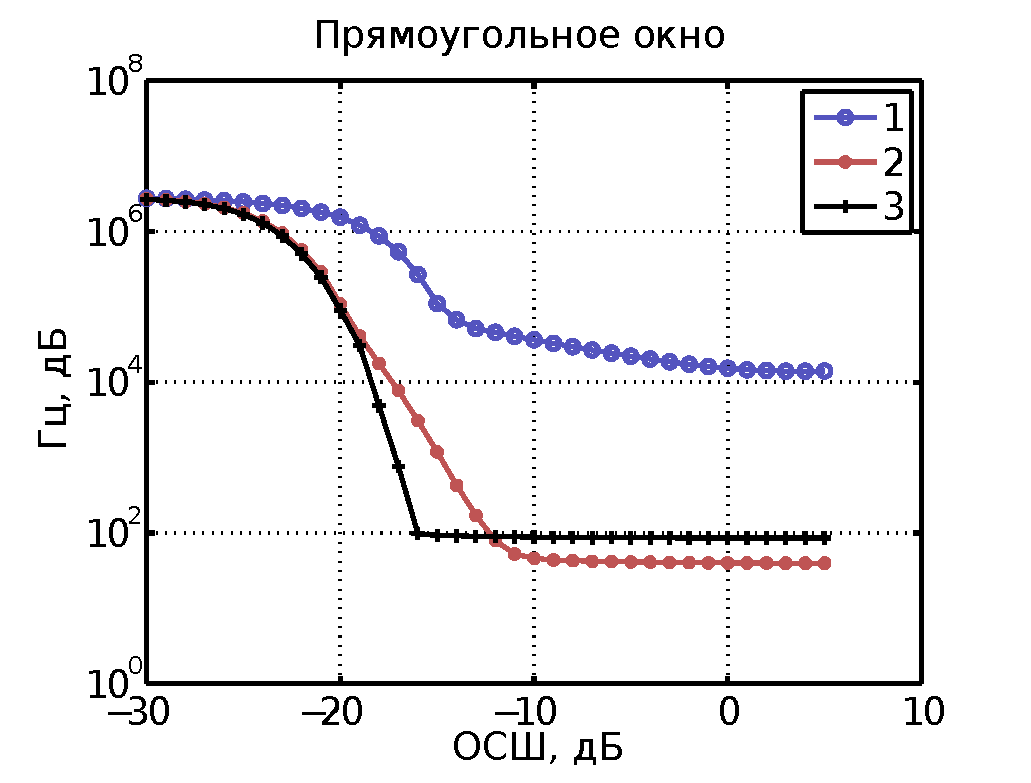
\includegraphics[width=1\linewidth]{fft2_rect_1_2_3.eps}}
	\caption{СКО оценки частоты.\\1 - одна итерация пересчета АКФ, 2 - две итерации пересчета АКФ, 3 - три итерации пересчета АКФ.}
	\label{pic:fft2_rect_1_2_3}
\end{figure}

Представляется интересным изучить влияние длинны блока нулей, дополняющий входную смесь, на СКО оценки частоты. Для решения данной задачи было проведено еще одно моделирование.
На Рис. \ref{pic:fft4_1} представлено моделирование для последовательности дополненной нулями до длинны ${4N}$ с применением различных оконных функций:
прямоугольного окна, окна Хемминга, окна Блекмана и окна Ханна при одной итерации уточнения АКФ.
\begin{figure}[h]
	\center\scalebox{0.8}{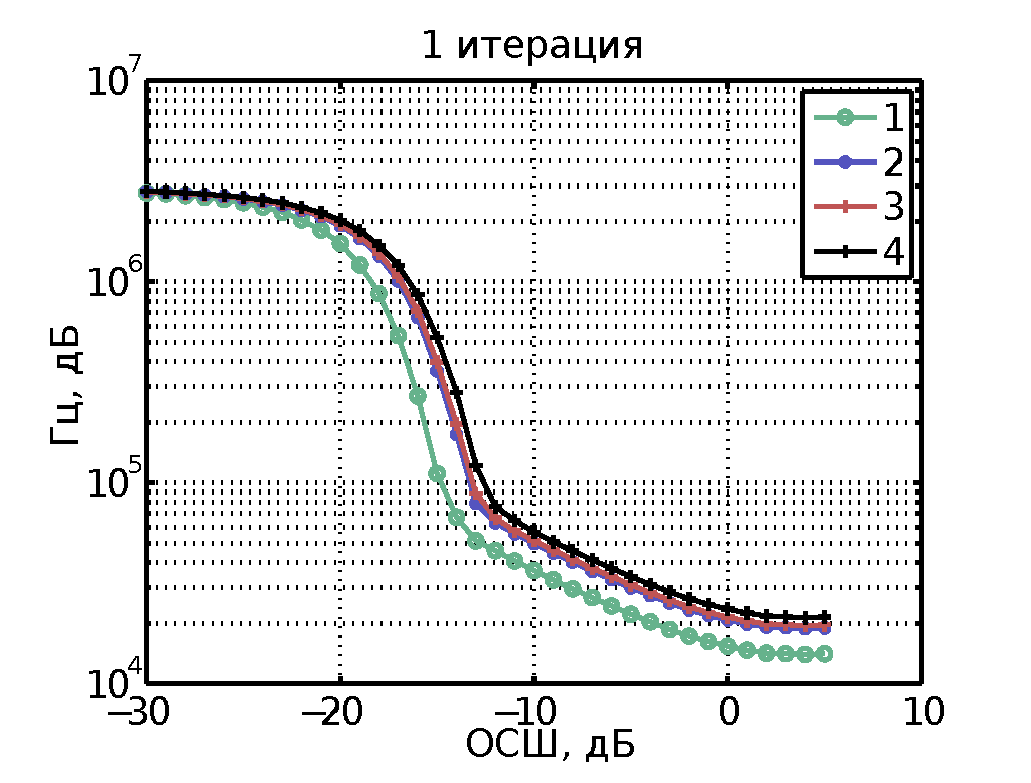
\includegraphics[width=1\linewidth]{fft4_1.eps}}
	\caption{СКО оценки частоты.\\1 - прямоугольное окно, 2 - окно Хемминга, 3 - окно Блекмана, 4 - окно Ханна.}
	\label{pic:fft4_1}
\end{figure}

На Рис. \ref{pic:fft4_2} представлено моделирование для последовательности дополненной нулями до длинны ${4N}$ с применением различных оконных функций:
прямоугольного окна, окна Хемминга, окна Блекмана и окна Ханна при двух итерациях уточнения АКФ.
\begin{figure}[h]
	\center\scalebox{0.8}{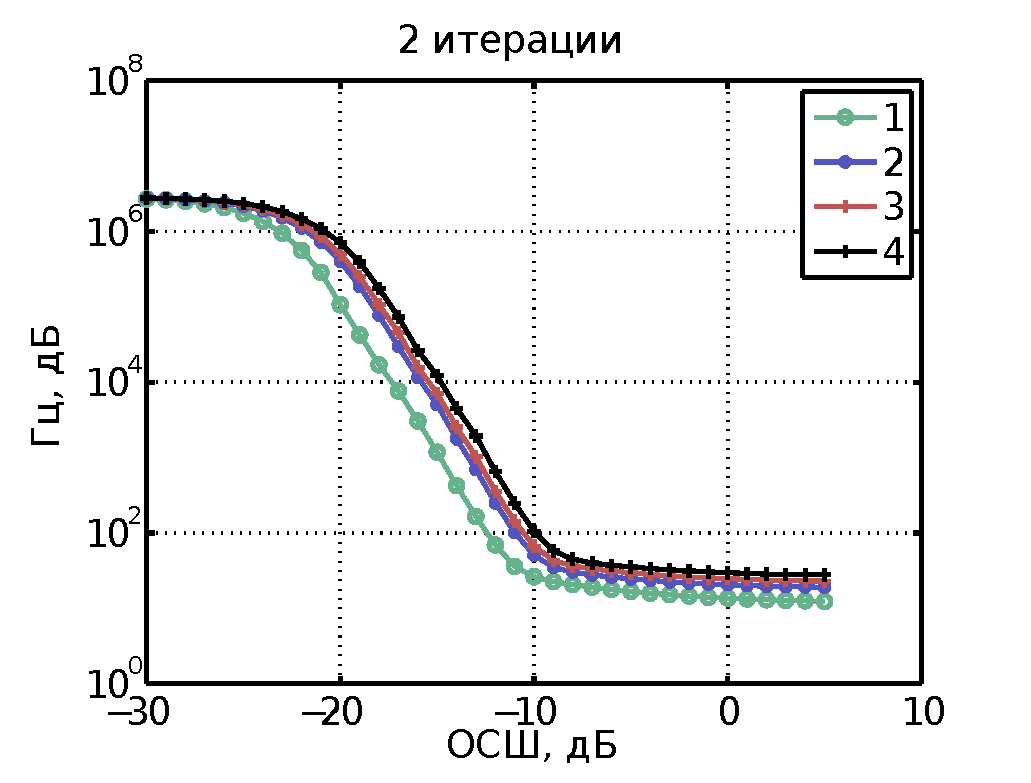
\includegraphics[width=1\linewidth]{fft4_2.eps}}
	\caption{СКО оценки частоты.\\1 - прямоугольное окно, 2 - окно Хемминга, 3 - окно Блекмана, 4 - окно Ханна.}
	\label{pic:fft4_2}
\end{figure}

На Рис. \ref{pic:fft4_3} представлено моделирование для последовательности дополненной нулями до длинны ${4N}$ с применением различных оконных функций:
прямоугольного окна, окна Хемминга, окна Блекмана и окна Ханна при трех итерациях уточнения АКФ.
\begin{figure}[h]
	\center\scalebox{0.8}{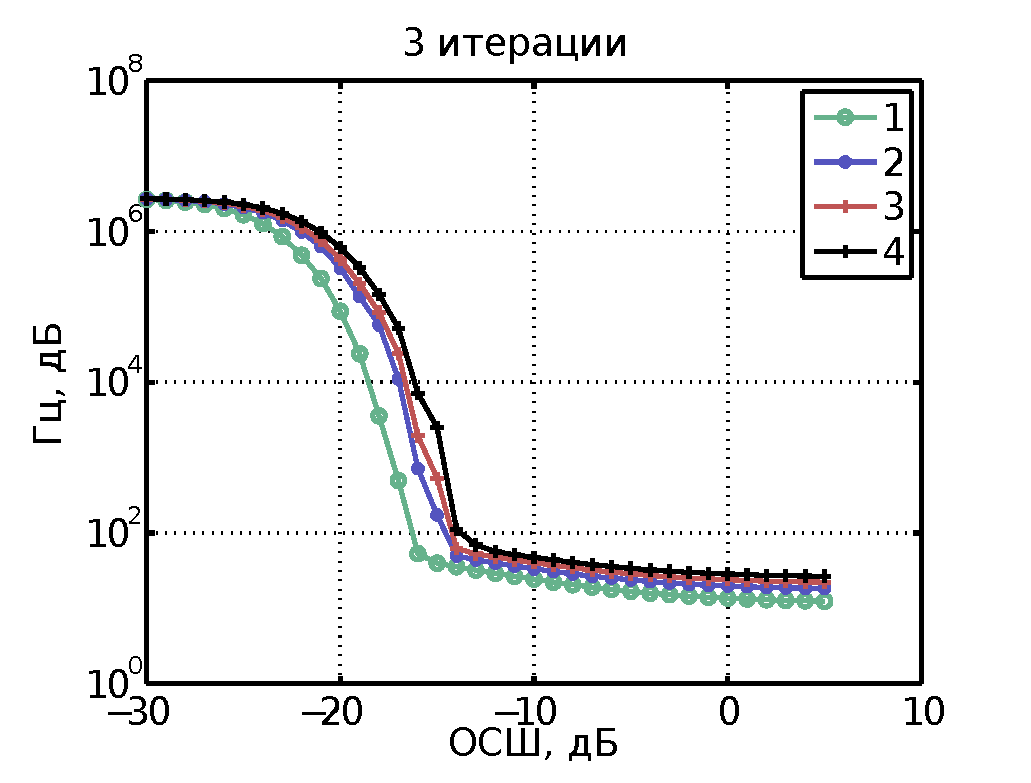
\includegraphics[width=1\linewidth]{fft4_3.eps}}
	\caption{СКО оценки частоты.\\1 - прямоугольное окно, 2 - окно Хемминга, 3 - окно Блекмана, 4 - окно Ханна.}
	\label{pic:fft4_3}
\end{figure}

Из Рис. \ref{pic:fft4_1}, \ref{pic:fft4_2}, \ref{pic:fft4_3} видно, что также как и в случае с длинной ${2N}$, лучшие результаты показывает подход с применением прямоугольного окна.
На Рис. \ref{pic:fft4_rect_1_2_3}
представлен график СКО оценки частоты для одной, двух и трех итераций уточнения АКФ с применением прямоугольного окна для блока данных, дополненного нулями до длинны ${4N}$.
Из графиков видно, что большее количество итераций уточнения позволяет более точно получать оценку на низких ОСШ, но в случае с длинной данных ${2N}$ оценки снижалась при
возрастании ОСШ при длине ${4N}$ данного эффекта не наблюдается.
\begin{figure}[h]
	\center\scalebox{1}{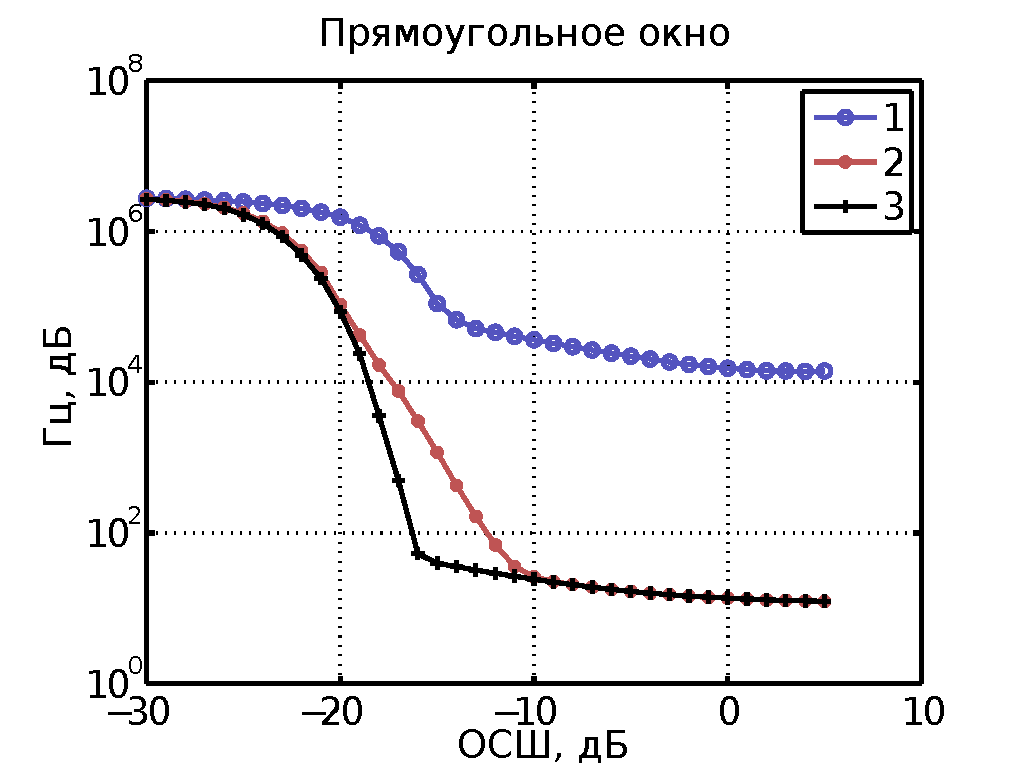
\includegraphics[width=1\linewidth]{fft4_rect_1_2_3.eps}}
	\caption{СКО оценки частоты.\\1 - одна итерация пересчета АКФ, 2 - две итерации пересчета АКФ, 3 - три итерации пересчета АКФ.}
	\label{pic:fft4_rect_1_2_3}
\end{figure}

%%%%%%
\section{Выводы по Главе 2}

\begin{itemize}
\item АКФ от гармонического сигнала является гармонический сигнал той же частоты, но с более высоким ОСШ.
\item Для повышения ОСШ при оценке АКФ можно итеративно пересчитывать АКФ тем самым увеличивая ОСШ до приемлемых значений.
\item Итеративное вычисление АКФ в Фурье домене позволяет существенно сократить вычислительные затраты.
\end{itemize}


\clearpage
